\subsection{The States HSQC experiment}
\label{subsec:theory__hsqc_states}

To illustrate the ideas developed in the previous section, we now turn our attention to two typical implementations of the 2D HSQC experiment, where both phase cycling as well as gradients are used to select for particular product operators.
\Cref{fig:hsqc_ph} shows an HSQC experiment where quadrature detection in the indirect dimension is performed using the States method.

\begin{figure}[htbp]
    \centering
    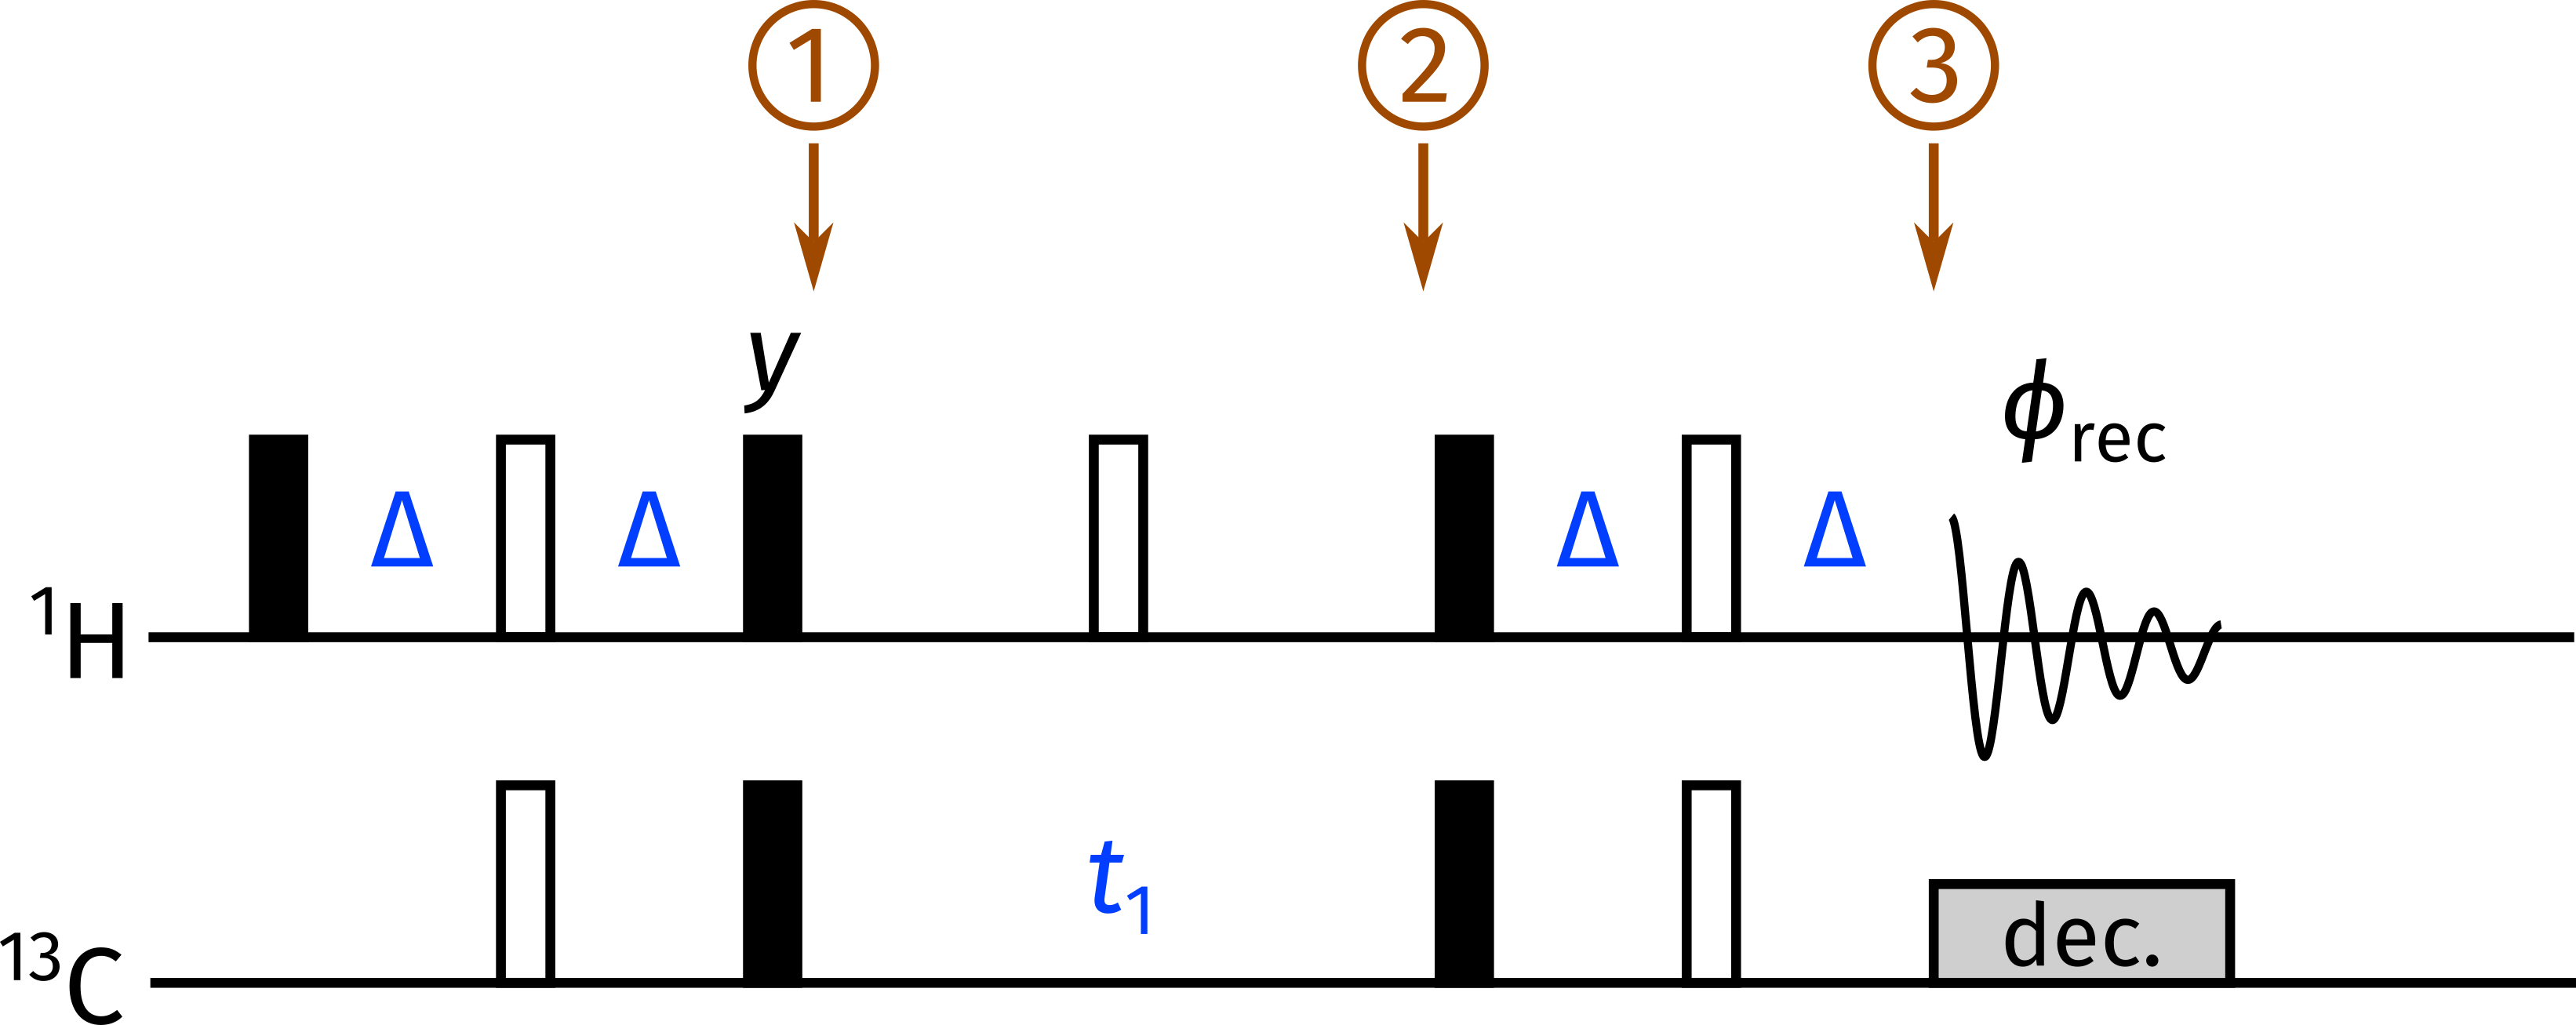
\includegraphics[]{pp/hsqc/ph.png}%
    \caption[Phase-sensitive HSQC pulse sequence with States method]{
        A typical HSQC pulse sequence utilising the States method for quadrature detection in $\omega_1$.
        The delay $\Delta$ is set to $1/(4 \cdot \oneJ{CH})$.
        To record the cosine-modulated dataset $s_\text{cos}(t_1, t_2)$, we set $\phi_1 = \phirec = (x, -x)$.
        The sine-modulated dataset $s_\text{sin}(t_1, t_2)$, on the other hand, is obtained using $\phi_1 = (-y, y)$ and $\phirec = (x, -x)$.
    }
    \label{fig:hsqc_ph}
\end{figure}

The HSQC experiment seeks to only detect protons directly bonded to \carbon{}; the signals from all other protons must be suppressed.
We first consider the simplest possible implementation of the HSQC, shown in \cref{fig:hsqc_ph}; as before, we will illustrate this with an $IS$ spin pair.
It can be shown that the equilibrium $S$-magnetisation cannot be transformed into observable $I$-magnetisation at the end of the sequence, so we will simply take $\rho_0' = I_z$.
Consider first the `basic' case where $\phi_1 = x$.
The \textit{preparation period} is just the same INEPT element as analysed in \cref{subsec:theory__inept}, so at point \circled{1} we already know that we have
\begin{equation}
    \label{eq:hsqc_ph_rho_1}
    \rho = -2I_zS_y.
\end{equation}
During $t_1$, the J-coupling is refocused, but the offset evolves to give:
\begin{equation}
    \label{eq:hsqc_ph_after_t1}
    \rho = 2I_zS_y\cos(\Omega_S t_1) - 2I_zS_x \sin(\Omega_S t_1),
\end{equation}
at point \circled{2}, bearing in mind that the $\angang{180}{x}(I)$ pulse inverts the $I_z$ component of both terms.
Immediately after this, the reverse INEPT element (the `mixing' segment) transfers the amplitude-modulated $2I_zS_y$ coherence $I_x$ for detection.
However, the $2I_zS_x$ term is turned into a mixture of unobservable zero- and double-quantum coherence, such that immediately before detection (point \circled{3}) we have:
\begin{equation}
    \label{eq:hsqc_ph_detection}
    \rho = I_x\cos(\Omega_S t_1) = \frac{1}{2}(I_+ + I_-)\cos(\Omega_S t_1).
\end{equation}
Performing the usual quadrature detection in the direct $t_2$ dimension gives us the desired cosine-modulated signal of
\begin{equation}
    \label{eq:hsqc_cos_signal}
    s_\text{cos}(t_1, t_2) = \frac{1}{2}\cos(\Omega_S t_1)\exp(\mi \Omega_I t_2),
\end{equation}
In a similar way, it can be shown that setting $\phi_1 = -y\/$ yields the following after $t_1$ (point \circled{2})
\begin{equation}
    \label{eq:hsqc_ph_after_t1_sin}
    \rho = 2I_zS_x\cos(\Omega_S t_1) + 2I_zS_y \sin(\Omega_S t_1),
\end{equation}
which after the reverse INEPT gives us the desired sine-modulated signal
\begin{equation}
    \label{eq:hsqc_sin_signal}
    s_\text{sin}(t_1, t_2) = \frac{1}{2}\sin(\Omega_S t_1)\exp(\mi \Omega_I t_2).
\end{equation}
These can be combined in the way described in \cref{subsec:theory__2dnmr} to yield an HSQC spectrum with double absorption-mode lineshapes $A_1(\Omega_S)A_2(\Omega_I)$.

This alone is not sufficient to obtain a high-quality HSQC spectrum, however.
Not every \proton{} spin in a molecule will share a one-bond coupling to a \carbon{} spin:  for example, in a natural-abundance sample, the HSQC experiment only detects around $1\%$ of \proton{} spins.
Even small artefacts arising from the remaining $99\%$ of proton magnetisation may have comparable intensity to the signals of interest.
We therefore need to suppress any unwanted peaks which might arise from this \textit{`bulk'} magnetisation.

The simplest way to do this is to perform (at least) a two-step phase cycle, where the pulse phase $\phi_1$ and receiver phase $\phirec$ are simultaneously inverted.
This has no effect on the desired signal (it picks up two minus signs which cancel out), but will lead to cancellation of any signal arising from the bulk magnetisation, which does not evolve under $H_\text{J}$ and therefore cannot be affected by the pulse on spin $S$.
Note the similarity to the INEPT phase cycling in \cref{subsec:theory__inept}, where we chose to cycle a pulse which the undesired pathway did not `experience': this is not the only possible choice, but is one that is conceptually simple to understand.
Naturally, this phase cycling must be carried out for both the cosine- and sine-modulated datasets.
In practice, even longer phase cycles are typically required to deal with experimental imperfections.
